\documentclass{article}

\usepackage{pdfcomment}
\usepackage[margin=1in]{geometry}
\usepackage{xcolor}
\usepackage{graphicx}
\usepackage{algorithm}
\usepackage{caption}
\usepackage{subcaption}
\usepackage{listings}
\usepackage{verbatim}
\usepackage{booktabs}
\usepackage{makecell}

\usepackage[flushleft]{threeparttable}

\newcommand{\note}[2]{\pdfmargincomment[color=yellow,author=#1,open=true]{#2}}
\newcommand{\todo}[1]{\color{red}\textbf{TODO:}#1\color{black}}
\newcommand{\reprozip}[0]{ReproZip}

\title{Numerical error propagation in the HCP structural pre-processing 
pipelines}
\title{Reprotool: a debugging tool to identify numerical errors 
and assess reproducibility of the neuroimaging pipelines}

\author{M. Ali Salari, Lalet Scaria, Gregory Kiar, Lindsay B. Lewis,
  Alan C. Evans, Tristan Glatard}

\begin{document}

\maketitle

\abstract{


Many experiments show that computational analysis results are still not 
completely reproducible. Although new technologies such as 
virtualization , version control systems , and provenance management 
tools provide more reliable environment and significantly improve the 
reproducibility crisis. 
In particular, computational environments are known to have an effect 
on the results produced by neuroimaging pipelines, presumably due to 
the creation, propagation and amplification of small numerical errors 
across the pipelines. Similarly, small perturbations that originated 
from computational environments including diverse operating systems, 
hardware categories, software version, etc. highlight the numerical 
errors.
However, the precise causes of such instabilities and the path along 
which they propagate in the pipelines are unclear.  We present a 
technique to identify the processes in the pipeline that create numerical 
errors along the execution, and we apply this technique to the HCP 
structural pre-processing pipelines.

\section{Introduction}

Research findings are expected to be reproducible to evaluate the 
authenticity and reliability of the claims.There are different 
terminologies for the terms reproducibility, repeatability, and 
replicability over the time. For example, the Association for Computing 
Machinery (ACM)~\cite{acm2016terminology} proposes three different 
definitions. From the ACM's points of view, repeatability is defined as 
repeating the computation by the same experimental setup including 
operator team, operating conditions, location, and measuring system. 
Replicability has almost the similar definition with repeatability 
which use the identical experimental conditions except performer team 
which means that an independent group can achieve the same results. 
Beside, reproducibility is measured by performing different 
experimental setup via different laboratory team independently. In this 
paper, we follow Peng's~\cite{peng2011reproducible} definition of 
reproducibility which is assessed by performing the experiment using 
the same data and the same analytic methods and expecting the same 
results. A reproducible study provides a context in which, one is able 
to get the consistence results to the original work. In addition, it 
enables others to use the existing work as a part of their 
experiments~\cite{plesser2018reproducibility}. It not only saves a 
great deal of time, but also contributes to focusing on the other 
parts.

Reproducibility of computational pipelines has been repeatedly 
investigated so far. The comparisons show that the analysis results are 
not completely reproducible across the small perturbations which have 
emerged by changing the execution environments including operating 
system, software and analysis method, and hardware configuration. There 
are different studies that discovered factors that introduce such tiny 
perturbations and consequently hamper the reproducibility of the 
experiments. In particular, Groenschild \emph{et al.} first identified 
the effect of operating systems on Freesurfer 
results~\cite{Gronenschild2012}. Similarly, the effect of OS is 
quantified in~\cite{Glatard2015} more specifically on some 
of the main neuroimaging pipelines including several FSL pipelines, 
CIVET and Freesurfer. The results of comparisons indicate a significant 
errors between analysis results of the same experiment on different 
operating system. 

It should be noted that \emph{error} is defined as the statistical 
differences between results of two experiments in this work. Moreover, 
the operating system is defined here as a consistent set of software 
packages organized in a trusted repository.

The operating system is not the only part of the computational 
environment that may hamper reproducibility. Many other computational 
factors including hardware configuration, software version, and 
parallelization techniques are reported~\cite{diethelm2012limits} as 
the main influential computing infrastructure on reproducibility. 

It has revealed that the majority of analysis results are not 
numerically reproducible because of arithmetic operations which is 
associated with the type of execution such as sequential or parallel 
executions, floating-point operations, different standard calculations 
like IEEE-754 or other standards, etc.

In order to overcome these issues and making reproducible analysis, a 
comprehensive solution requires which not only encapsulates and 
re-executes all the software/hardware dependencies but also fixes the 
numerical instabilities. Therefore, we introduce a framework to 
identify the processes in the pipeline which are responsible for such 
numerical errors along the execution. In this paper, the execution 
results of the pipelines across different operating systems are 
considered to find out the cause of the reproducibility issues using an 
interposition techniques.

Figure~\ref{fig:overview} illustrate an overview of the proposed 
technique. First, we execute pipelines in a consistence environment 
using docker container and Boutiques framework. In the next step, the 
origin of errors, processes that make differences, are detected through 
a classification approach. Processes are classified by several 
modifications iteratively and finally, it creates corresponding process 
graph of the pipeline execution. We will explain each step in detail in 
the following sections.

\begin{figure}[H]
\centering
  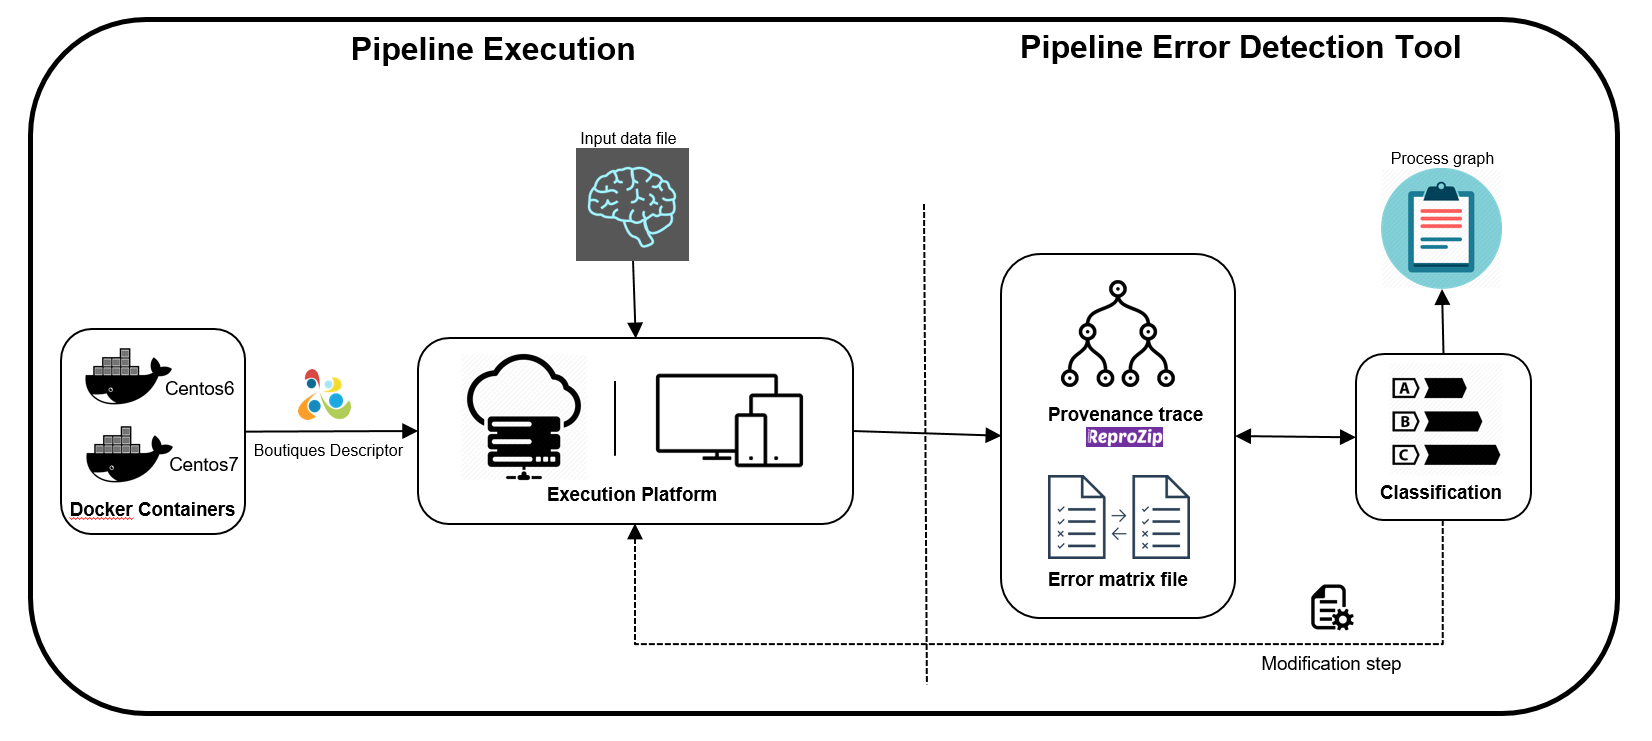
\includegraphics[scale=0.5]{images/overview.png}
  \caption{An overview of proposed technique.}
  \label{fig:overview}
\end{figure}

\paragraph{} The reminder of this paper explains the proposed debugging tool in two 
parts. First, the execution environment of the pipelines and then the 
classification procedure of the processes are clarified. We describe 
the HCP preprocessing pipelines as a popular neuroimaging pipelines to 
test and apply reprotool. Finally, we report the analytic process which 
are responsible for the errors in the pipelines.

\section{Processing Environment}

We build the containerized version of pipelines for each operating 
system using docker technology which encapsulated whole the pipeline 
dependencies. The docker images consists of an specific computing 
environment such as operating system version, hardware configuration, 
software version, etc. Furthermore, derived images can be stored on 
the dockerhub repositories and be version controlled in the same way as 
the analysis code so that the exact same environment can be used to run 
an experiment.

To simplify computational reproducibility of the analysis, we execute 
docker images using Boutiques framework based on the command-line 
descriptions~\cite{glatard2017boutiques}. The Boutiques descriptor 
specifies the parameters and implementation of the experiment, and the 
invocation schema describes the parameter values such as input/output 
data path.

We processed subjects twice in every condition to identify possible 
\emph{intra-condition} errors coming from the use of pseudo-random 
numbers or other external factors. To further ensure that the observed 
errors are caused by operating system updates (\emph{inter-os 
differences}) and not by other factors, we implemented the following 
sanity checks:

\begin{itemize}

\item The file checksums of every subject are computed before and after 
processing to detect potential corruption during file transfers and 
other manipulations. 
\item The checksum of the Docker container images is recorded with
  every execution to identify any unintentional package update. In 
  addition, the list of packages with versions is printed by every task 
  and checked for consistency.
\item Hardware information is captured to make sure that errors are
  not coming from different CPU architectures.
\item Every task is executed on its own copy of the data to ensure
  that input data is not modified by the pipeline. 
\end{itemize}
	

\section{Measuring Differences}

We compute a file difference matrix between files produced for every 
subject in every operating system based on MD5 
checksums~\cite{md51992url} as in~\cite{Scaria2017}. MD5 is suitable to 
identify incidental file differences, although it is not 
cryptographically secure. Files produced only in some subjects or in 
some operating systems were left out.

In addition, we are able to quantify errors in the image files using 
the Dice coefficient and normalized root mean square error (NRMSE) 
computed as follows:

\begin{center}
\begin{equation}
RMSE = {\sqrt {\frac{1} {n}{\sum\limits_{t = 1}^n {(\hat{y}_{t} - {y}_{t} } })^{2} } }
\end{equation}
\end{center}

\begin{center}
\begin{equation}
NRMSE = {\frac{RMSE} {y_{max} - y_{min}}}
\end{equation}
\end{center}

\section{Pipeline Analysis: Characterizing Errors}

Once errors between conditions are quantified, we automatically
identify the steps in the pipeline responsible for such differences.
We use the \reprozip tool~\cite{Chirigati2016} to record: (1) the tree of
processes executed by the pipeline and (2) the list of files read and
written by each process. This information is collected by system call
interceptions, through the \texttt{ptrace} Unix system call, and
stored in a \texttt{SQLite} database. The database stores information
on all the processes which are created by the \texttt{clone()} or
\texttt{fork()} system calls. It also records the files opened by each
process (in read, write or execution mode), including the result files
and the temporary files.

We reconstruct the tree of processes starting from the first process 
created by the pipeline and identifying its child processes as the ones 
that were created through \texttt{clone()} or \texttt{fork()}. We 
create a process graph from this tree by adding edges corresponding to 
file dependencies between processes. A file dependency is defined 
between processes A and B if a file written by A is read by B. 
Figure~\ref{fig:simple_script} shows an example of a process graph 
constructed at this stage.

\medskip
\noindent
\begin{minipage}[]{.5\linewidth}
  \centering
  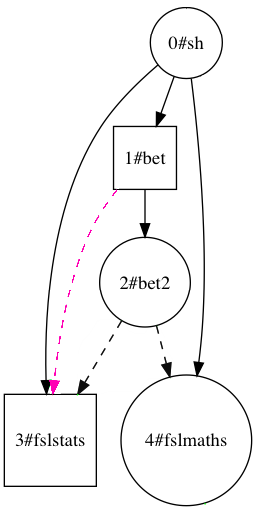
\includegraphics[scale=0.2,width=.4\linewidth]{images/simple_graph}
%  \captionof{figure}{This is a figure caption.} \label{myfig1}
\end{minipage}
\begin{minipage}[]{.3\linewidth}
\small\captionof{algorithm}{sample script of a process graph}\label{sample_script}
{\scriptsize
\begin{verbatim}
#!/bin/bash
if [ # !=1 ]
then
    echo "usage: 0 <inputimage.nii.gz>"
    exit 1
fi
input_image=$1
bet_output="$(basename ${input_image} .nii.gz)_brain.nii.gz"
bet_output_binarized="$(basename ${input_image} .nii.gz)_brain_bin.nii.gz"

bet ${input_image} ${bet_output} > bet_temp.out
echo "Voxels / Volume in brain mask:"
fslstats ${bet_output} -V
fslmaths ${bet_output} ${bet_output_binarized}
echo "Voxels / Volum in binarized brain mask:"
\rm bet_temp.out
\end{verbatim}
}
\end{minipage}
\captionof{figure}{Process graph constructed from an example brain extraction
	script. Every node in the graph is labeled using (1) a process id 
	created by our reconstruction, (2) the name of the executable run 
	by the process. Processes that read or write temporary files are 
	represented with squares; other ones with circles. Plain edges 
	represent the process tree (\texttt{fork()} or \texttt{clone()} 
	system calls). Dashed edges represent file dependencies: temporary 
	files are in yellow and result files are in green.} 
	\label{fig:simple_script}
\medskip

A different process graph may be produced for every subject in every 
execution condition. Among our dataset, we identified 4 types of 
subjects with different numbers of T1w and T2w images. We verified that 
the process graphs were identical for all subjects of the same type, 
for all execution conditions \todo{Check that}. The remainder of the 
analysis is done separately for each subject type.

Cycles may be present in the process graph in case a file was written 
by more than one process. We remove such cycles by removing file edges 
between processes A and B when A's process creation timestamp is 
posterior to B's or when A=B. Indeed, such edges cannot happen in 
practice unless A and B were running concurrently, which we assume is 
not the case (we also checked that on the workflow we tested). 

\paragraph{} In the next step, we classify the processes into three 
categories based on the process graph and the error matrix file 
mentioned in the previous Section:
\begin{enumerate}
\item Processes that read files that do not have errors and write files that do not 
have errors are \emph{transparent} (Figure~\ref{fig:processes}.a).
\item Processes that read files 
that do not have any error but write files that have errors 
\emph{create} errors in the pipeline (Figure~\ref{fig:processes}.b).
\item Processes that read files 
that have errors and write files that do not have errors \emph{remove} 
errors from the pipeline (Figure~\ref{fig:processes}.c).
\item Processes that read files that have errors and write files that also have errors are 
\emph{unknown} (Figure~\ref{fig:processes}.d).
\end{enumerate}

\begin{figure}[H]%\centering
    \begin{subfigure}{0.15\textwidth}
        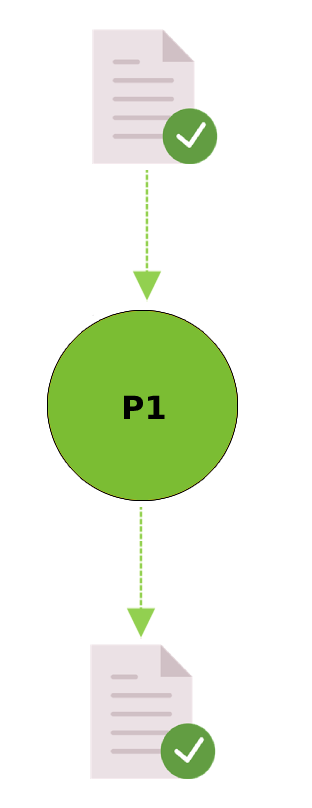
\includegraphics[scale=0.35]{images/green.png}
        \caption{Transparent}
        \label{fig:green}
    \end{subfigure}
\hfill%\hfil
    \begin{subfigure}{0.15\textwidth}
    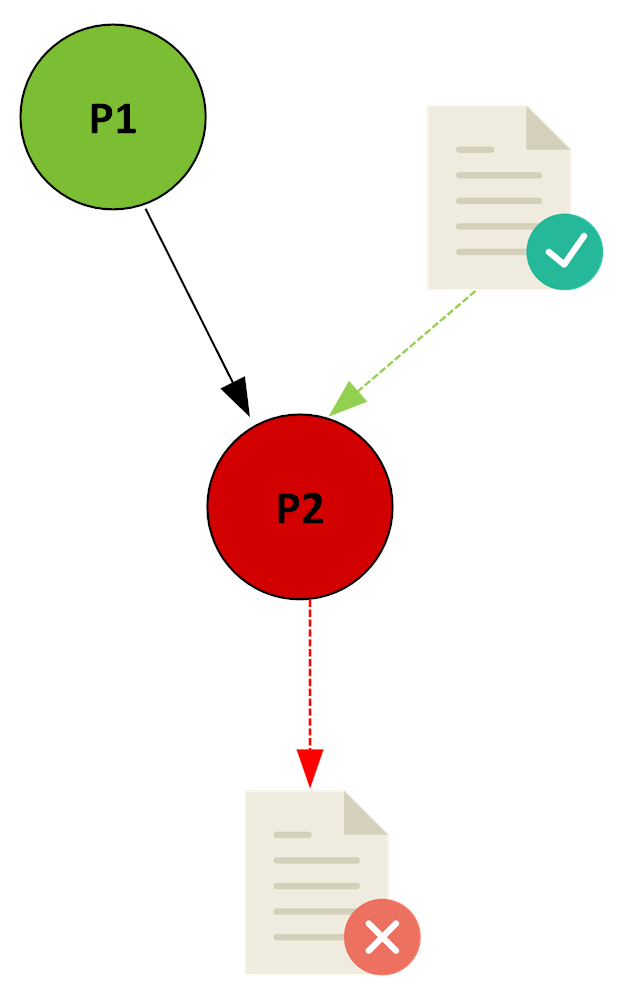
\includegraphics[scale=0.35]{images/red.png}
    \caption{Creates error}
    \label{fig:red}
\end{subfigure}
\hfill%\hfil
    \begin{subfigure}{0.15\textwidth}
    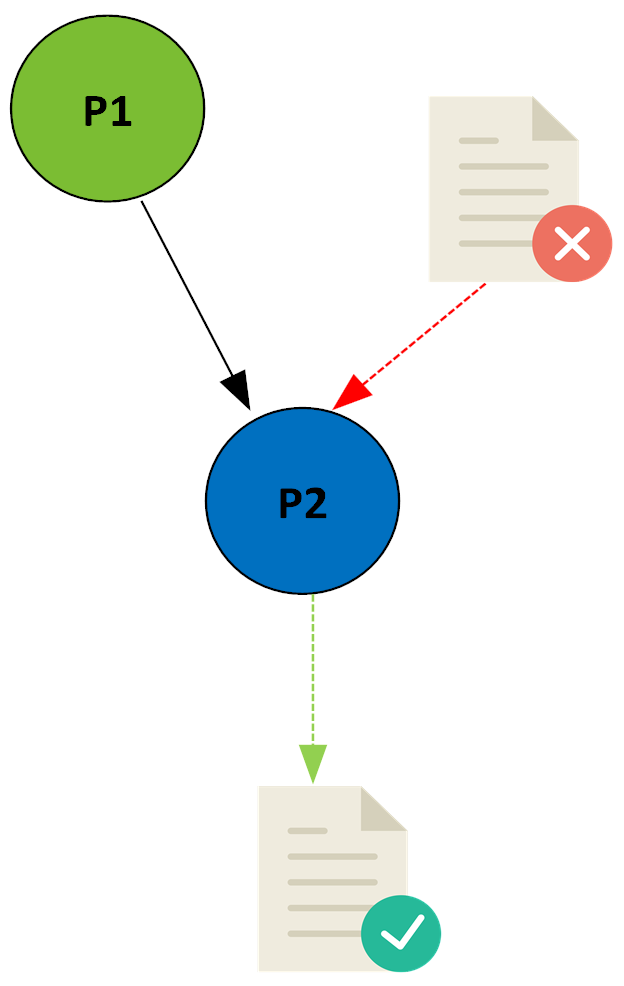
\includegraphics[scale=0.35]{images/blue.png}
    \caption{Removes error}
    \label{fig:blue}
\end{subfigure}
\hfill%\hfil
    \begin{subfigure}{0.15\textwidth}
    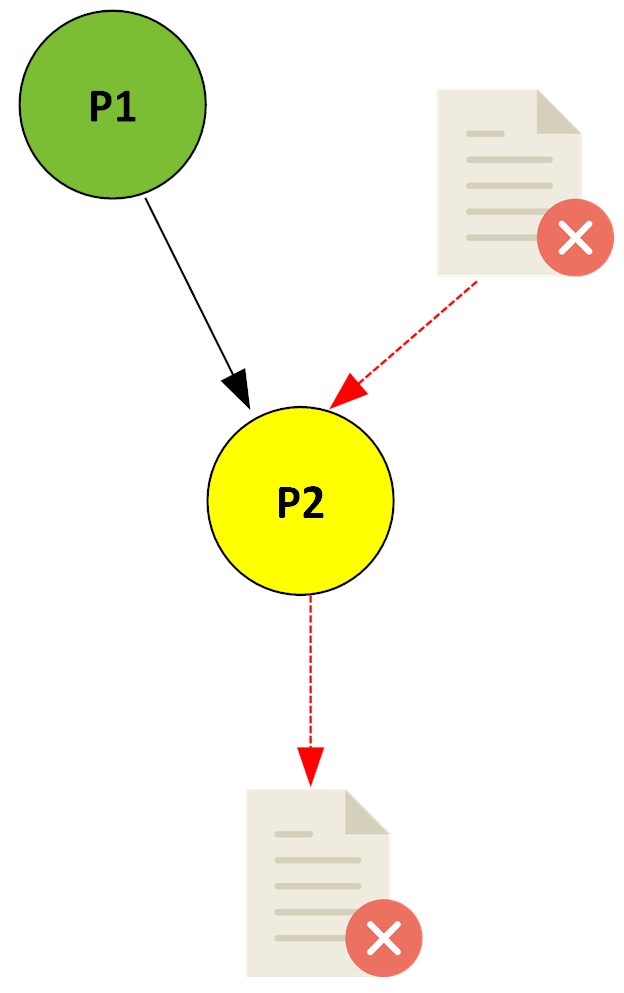
\includegraphics[scale=0.35]{images/yellow.png}
    \caption{Unknown}
    \label{fig:yellow}
\end{subfigure}
    \caption{Different type of classified process based on the input/output files.
  Dashed edges refer to the file dependencies between processes A and B 
  if a file written by A is read by B. Solid black edges refer to the 
  relationship between parent and child processes.}
    \label{fig:processes}
\end{figure}

\paragraph{Challenge1:} The classification of processes that read or 
write temporary files is uncertain when these files are deleted during 
the execution. To address this issue, we replace every process P that 
writes temporary files with a modification of P that first calls P and 
then backs up all its output files to a read-only directory. This 
replacement is done by modifying the Unix PATH variable to point to a 
directory containing the modified versions of the processes. This 
solution does not cover the temporary files that are removed by P 
itself; this is not a problem since these files do not play any role in 
the subsequent steps of the pipeline, by definition.

\paragraph{Challenge2:} Files written by multiple processes also lead 
to unknown classification labels. To address this issue for a file F 
written by processes in \textbf{P} = \{$P_{1}$, \ldots $P_{n}$\}, we 
(1) check that processes in \textbf{P} do not write concurrently to F, 
(2) we establish an order on \textbf{P} based on the creation timestamp 
of the processes, (3) we replace ever process $P_{i}$ in \textbf{P} by 
a wrapper that first calls $P_{i}$ and then backs up F to a read-only 
directory. Thus, multiple versions of F are saved and used in the 
analysis.

\paragraph{Challenge3:} Another challenge is to classify processes that 
read files that have errors and write files that also have errors. In 
such situations, it is not possible to determine from the pipeline 
results whether the process created errors, removed some errors, or was 
transparent. We label such processes \emph{unknown}. To address this 
issue, we developed an iterative approach that consists of the 
following steps: 

\begin{enumerate}
  \item Run the pipeline in conditions 1 and 2; classify the
    processes as \emph{transparent}, \emph{create errors},
    \emph{remove errors} or \emph{unknown}.
  \item If there are \emph{unknown} processes then: replace each process P that create errors by a process Q that
    copies the results produced by process P in condition 1 to the pipeline output in condition 2.
  \item Repeat steps 1 and 2 until there is no \emph{unknown} process left.
\end{enumerate}

The replacement of process P at step 2 is done by replacing P with a 
custom script produced by step 1. This custom script copies the results 
obtained in condition 1 if it is invoked with the arguments of a 
process that created errors, and calls P's original executable 
otherwise. The replacement is done through the PATH variable, as 
before. This algorithm converges to a process graph without any 
\emph{unknown} process after a finite number of iterations.

\begin{figure}[H]
\centering
  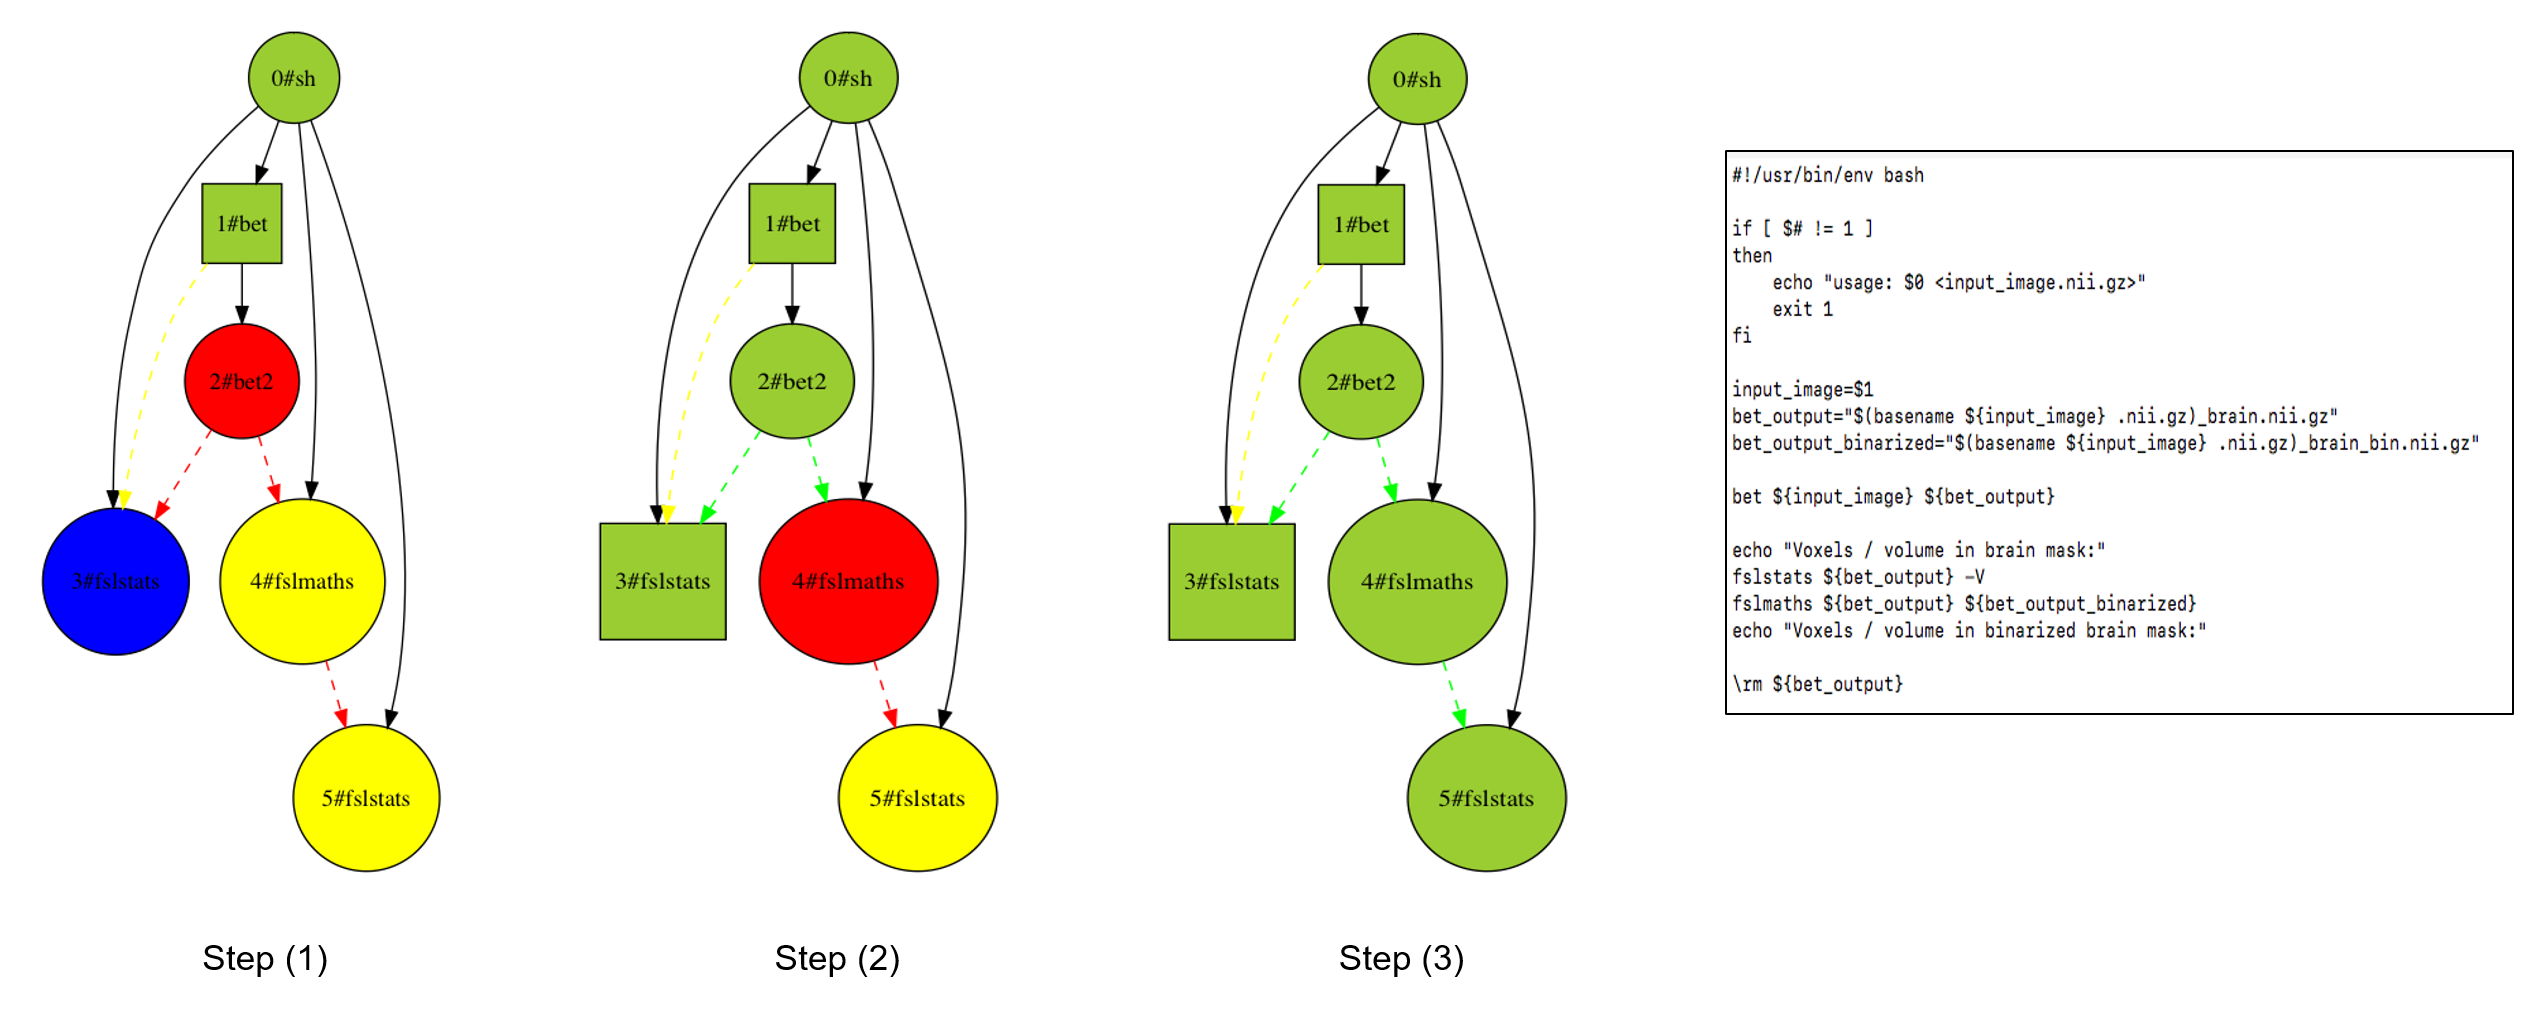
\includegraphics[scale=0.5]{images/iterative_modif}
  \caption{iteration of proposed modification.}
  \label{fig:iterations}
\end{figure}

Figure~\ref{fig:iterations} illustrates our iterative classification 
process for the example in Figure~\ref{fig:graph-example}. At every 
step, processes that created errors are shown in red, processes that 
removed errors are in blue, processes that propagated errors are in 
yellow, and other processes (transparent processes) are in green. As in 
Figure~\ref{fig:graph-example}, plain black edges represent the process 
tree and dashed edges represent file dependencies: green edges 
represent files with no errors, while red edges represent files with 
errors. Temporary files are not represented because they have been 
backed up as previously described.

The three steps in Figure~\ref{fig:iterations} correspond to the 
iterations of the classification algorithm At step one \texttt{2\#bet2} 
is classified as error creator (red) as it produced files with errors 
from files without error. \texttt{3\#fslstats} is classified as error 
remover (blue) as it produced files without errors from files with 
errors. \texttt{4\#fslmaths} and \texttt{5\#fslstats} are classified as 
unknown (yellow) as they produce files with errors from files with 
errors.

At step 2, the files produced by \texttt{2\#bet2} in the tested 
condition are replaced with the files produced by \texttt{2\#bet2} in 
the other condition. \texttt{3\#fslstats} is now classified as 
transparent, \texttt{4\#fslmaths} is now classified as error creator 
and \texttt{5\#fslstats} is still unknown.

 At step 3, the files produced by \texttt{4\#fslmaths} in the tested 
 condition are replaced with the files produced by \texttt{4\#fslmaths} 
 in the other condition. \texttt{5\#fslstats} is now transparent.
 
 As a result of those 3 steps, the final process classification is: 
 \texttt{2\#bet2} and \texttt{4\#fslmath} are error creators (red), 
 \texttt{3\#fslstats} is error remover (blue) and the other processes 
 are transparent.

The process graphs of real pipelines are much larger than the one in 
Figure~\ref{fig:iterations}. To represent such large graphs, we 
summarize them by (1) building subgraphs for every interesting node 
(e.g. red and blue nodes with their children) (2) building connected 
components in the absence of interesting nodes for the remaining nodes 
in the process graph. Each node in the summarized graph represent 
either a shrinked interesting subgraph or connected component and edges 
represent any connection between two shrinked nodes.



\section{HCP Minimal preprocessing Pipelines}


The Human Connectome Project (HCP)~\cite{glasser2013minimal} developed 
a set of pipelines to help extraction of structural, functional or 
diffusion MRI data across a large set of high resolution MR images. 
These pre-processing pipelines create results that are available in 
standard volume and combined surface and volume spaces which makes it 
easier for researchers to compare the images across the neuroimaging 
spectrum. 

We focused on HCP structural pre-processing pipelines to (1)quantify 
the effect of OS on HCP pre-processing pipelines (2) identify the 
process(es) in the pipelines that are responsible for such effects.

\paragraph{Structural Pre-processing Pipelines} The structural 
pre-processing consists of PreFreeSurfer, FreeSurfer and 
PostFreeSurfer~\cite{glasser2013minimal}. In this paper, we analyzed two 
pipelines, PreFreeSurfer and FreeSurfer. 

PreFreeSurfer consist of various steps including correction of MR 
gradient nonlinearity distortions, align the T1w and T2w images using 
FSL FLIRT, Align native space to MNI template using ACPC and FSL FLIRT, 
brain extraction usin FSL FLIRT and FNIRT to MNI template, register T2w 
to T1w using FLIRT's BBR, perform a bias field correction, and register 
the subject's native structural space to MNI space. 

FreeSurfer steps are downsample the images if it exceeds the resolution limit, 
generation of white matter surface using a segmentation of downsampled image, 
adjust T1w colum intensity and white matter surface position based on 0.7mm 
T1w images, fine tune the T2w to T1w registration using FreeSurfer's BBRegister 
algorithm, accurately place the white and pial surface with high-resolution 0.7mm 
T1w and T2w data, these inputs are fed back into recon-all at each stage. 

We randomly selected 10 subjects from the HCP data release S500 which 
are described in table~\ref{table:data}.

\begin{table}[H]\hspace*{-1cm}
\centering
\begin{threeparttable}
\caption{An overview of the HCP data (Humman Connectome DB).}

\begin{tabular}{@{}llllll@{}}
\toprule
Subject & Release & Acquisition & Gender & Age      & Subj\_Type   \\ \midrule
103515  & Q1      & Q02         & F      & 26-30    & type1         \\
105216  & Q3      & Q03         & M      & 26-30    & type4         \\
103414  & Q2      & Q02         & F      & 22-25    & type1         \\
125525  & Q1      & Q01         & F      & 31-35    & type1         \\
142828  & Q1      & Q01         & M      & 31-35    & type1         \\
129533  & Q3      & Q04         & F      & 31-35    & type1         \\
103818  & Q1      & Q01         & F      & 31-35    & type3         \\
133928  & Q2      & Q03         & M      & 26-30    & type3         \\
148032  & Q3      & Q03         & F      & 31-35    & type2         \\
139637  & Q2      & Q03         & F      & 31-35    & type1         \\ \bottomrule
\end{tabular}
\begin{tablenotes}
      \small
      \item *Subj\_Type refers to the graph topology type of the subjects,
      we will discuss further on the next sections.
\end{tablenotes}
\end{threeparttable}
\label{table:data}
\end{table}


\section{Results}

We executed the pipelines using Docker containers to simplify the 
deployment of different operating system versions on execution 
platforms. The Docker images were built for the HCP pre-processing 
pipelines v3.19.0 (PreFreeSurfer and FreeSurfer) in 
CentOS 6.8 and CentOS 7.2. Docker images are available on DockerHub for 
reuse \url{https://hub.docker.com/r/bigdatalabteam/hcp-prefreesurfer/}. 
We collected the provenance trace (tree of executed processes and files 
accessed in read or write mode) for each type of 
subjects(Table~\ref{table:data}) using system-call interception as 
provided by the \reprozip tool~\cite{Chirigati2016}.

\paragraph{} Two types of errors can occur in the subjects due to the 
errors in the operating systems. One is inter-OS error caused by the 
operating system library updates and the other type, intra-OS errors 
occurs as a result of the pseudo-random processes used in the 
pipelines. An example of a pseudo-random process function is, a random 
number generator that would get initialized using a seed state. the 
proposed method can be used to identify both kind of errors. The files 
that are common to all the subjects only are taken into consideration 
for comparison. The first step is identification of files with 
differences in their checksums. This is identified using the checksums 
that are recorded after the processing. Intra-OS errors are identified 
using the run-number added as the suffix for the conditions. For 
example, the two batches of subjects processed under the same condition 
(CentOS6) are stored as run-1 and run-2. The files belonging to the 
subjects stored under the above mentioned conditions are treated as 
intra-OS runs.

\subsection{Inter-OS differences}


\paragraph{Binary differences}

In a previous study~\cite{Scaria2017}, we showed that pre-processing 
pipelines of the Human Connectome Project~\cite{Glasser2013} were 
sensitive to operating system variation so that Figure 
\ref{fig:tissue_class} illustrates the binarized errors after brain tissue 
segmentation process in PreFreeSurfer. In addition, 
Figure~\ref{fig:fnirt_result} shows the same errors occurred in 
non-linear registration process between CentOS6 and CentOS7. 
Figure~\ref{fig:pipeline_errors}.a.


\begin{figure}[H]
\centering
  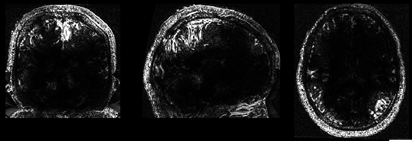
\includegraphics[scale=0.6]{images/fnirt_result.png} 
  \caption{Absolute errors between FNIRT results from PreFreeSurfer 
  (T2w\_acpc\_to\_MNI\_nonli.nii.gz), subject 104820 (centos6 vs. 
  centos7)~\cite{Scaria2017}. } 
  \label{fig:fnirt_result}
\end{figure}

\begin{figure}[H]
%  \includegraphics{brain\_classification}
\centering
  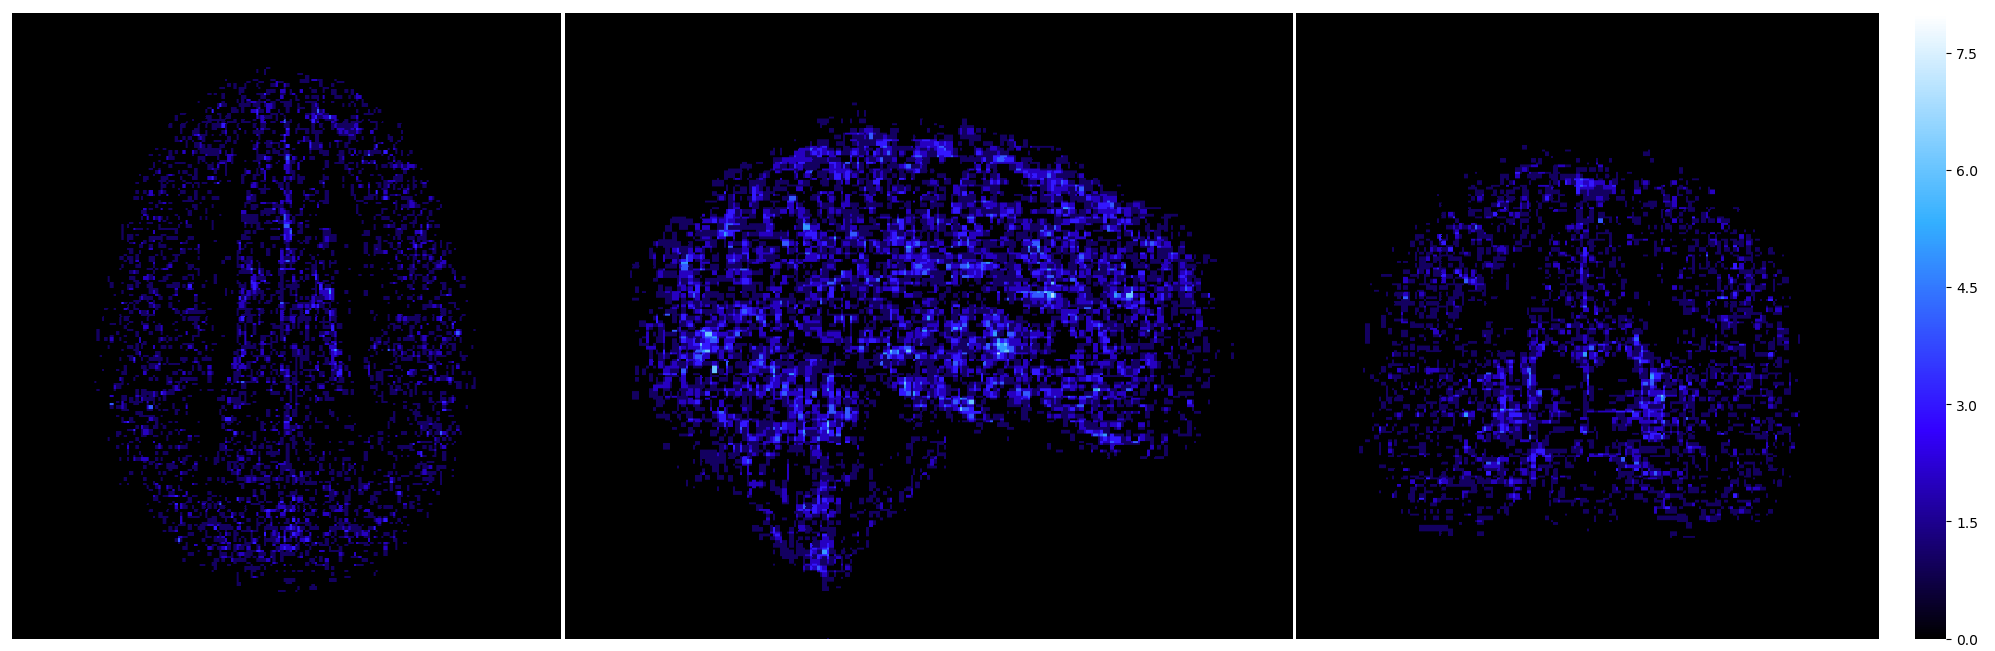
\includegraphics[scale=0.18]{images/brain_classification.png} 
  \caption{Binarized error between brain segmentation results from 
  FreeSurfer, subject 105216 (CentOS6 vs. CentOS7)~\cite{Scaria2017}.
    } 
  \label{fig:tissue_class}
\end{figure}

\subsection{Pipeline analysis}

We identified processes that introduce errors in both PreFreeSurfer and 
FreeSurfer pipelines. The result of our experiment is described in the 
following paragraphs.

\paragraph{PreFreeSurfer.} Among the 117 data files produced by 
PreFreeSurfer, 21 did not have any error for any subject, 92 had errors 
for all subjects and 4 had errors for 3 subjects only. 

Figure \ref{fig:summarized-graph} shows the annotated provenance graph 
of the PreFreeSurfer pipeline executed on CentOS6 and CentOS7. Each 
node in the graph represent an executed process in the pipeline. 
Processes that created errors are shown in red, processes that removed 
errors are in blue, and other processes are in green.  Squares denote 
processes for which the classification is uncertain, due to temporary 
files that were removed during the execution. Black edges link 
sub-processes to their parents while dashed edges denote file 
dependencies between processes (green edges: files with no errors; red 
edges: files with errors; yellow edges: temporary files).

The processes that introduce errors in PreFreeSurfer along with the 
number of occurrences are depicted in Figures~\ref{fig:pfs_table, 
fig:pfs_chart} including linear registration with “\emph{FLIRT}” (in 
ACPC Alignment, BrainExtraction, DistortionCorrection, 
AtlasRegistration), non-linear registration with “\emph{FNIRT}” (in 
BrainExtraction and AltasRegistration), image warping with 
“\emph{new\_invwarp}” (in BrainExtraction and AtlasRegistration).  In 
addition, errors were observed in image mean and standard-deviation 
computations with “\emph{fslstats}” (in BiasFieldCorrection), and in 
masked image extrapolation with “\emph{fslmaths}” (in 
BiasFieldCorrection).  Besides, transformation format conversion with 
“\emph{convertwarp}” (in DistortionCorrection) was able to remove 
errors.

\begin{figure}[H]
\centering
  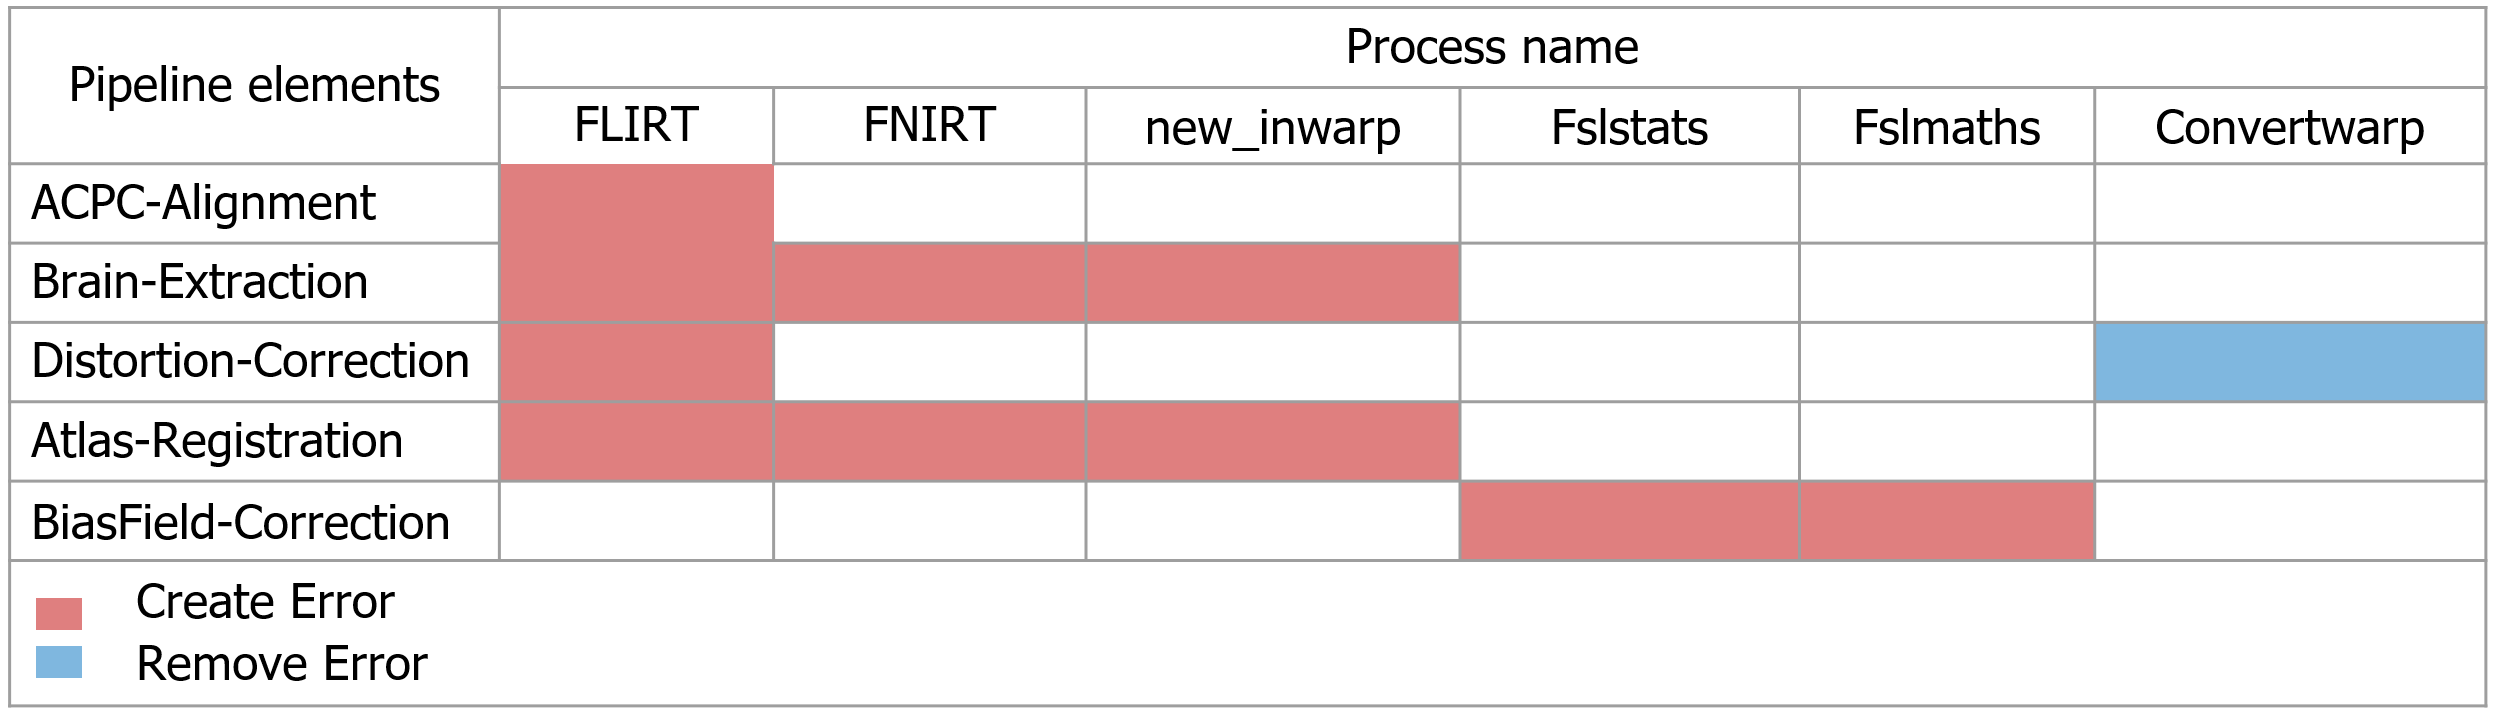
\includegraphics[scale=0.5]{images/pfs_table.png}
  \caption{Process name along with the pipeline elements that introduce errors.}
  \label{fig:pfs_table}
\end{figure}

\begin{figure}[H]
\centering
  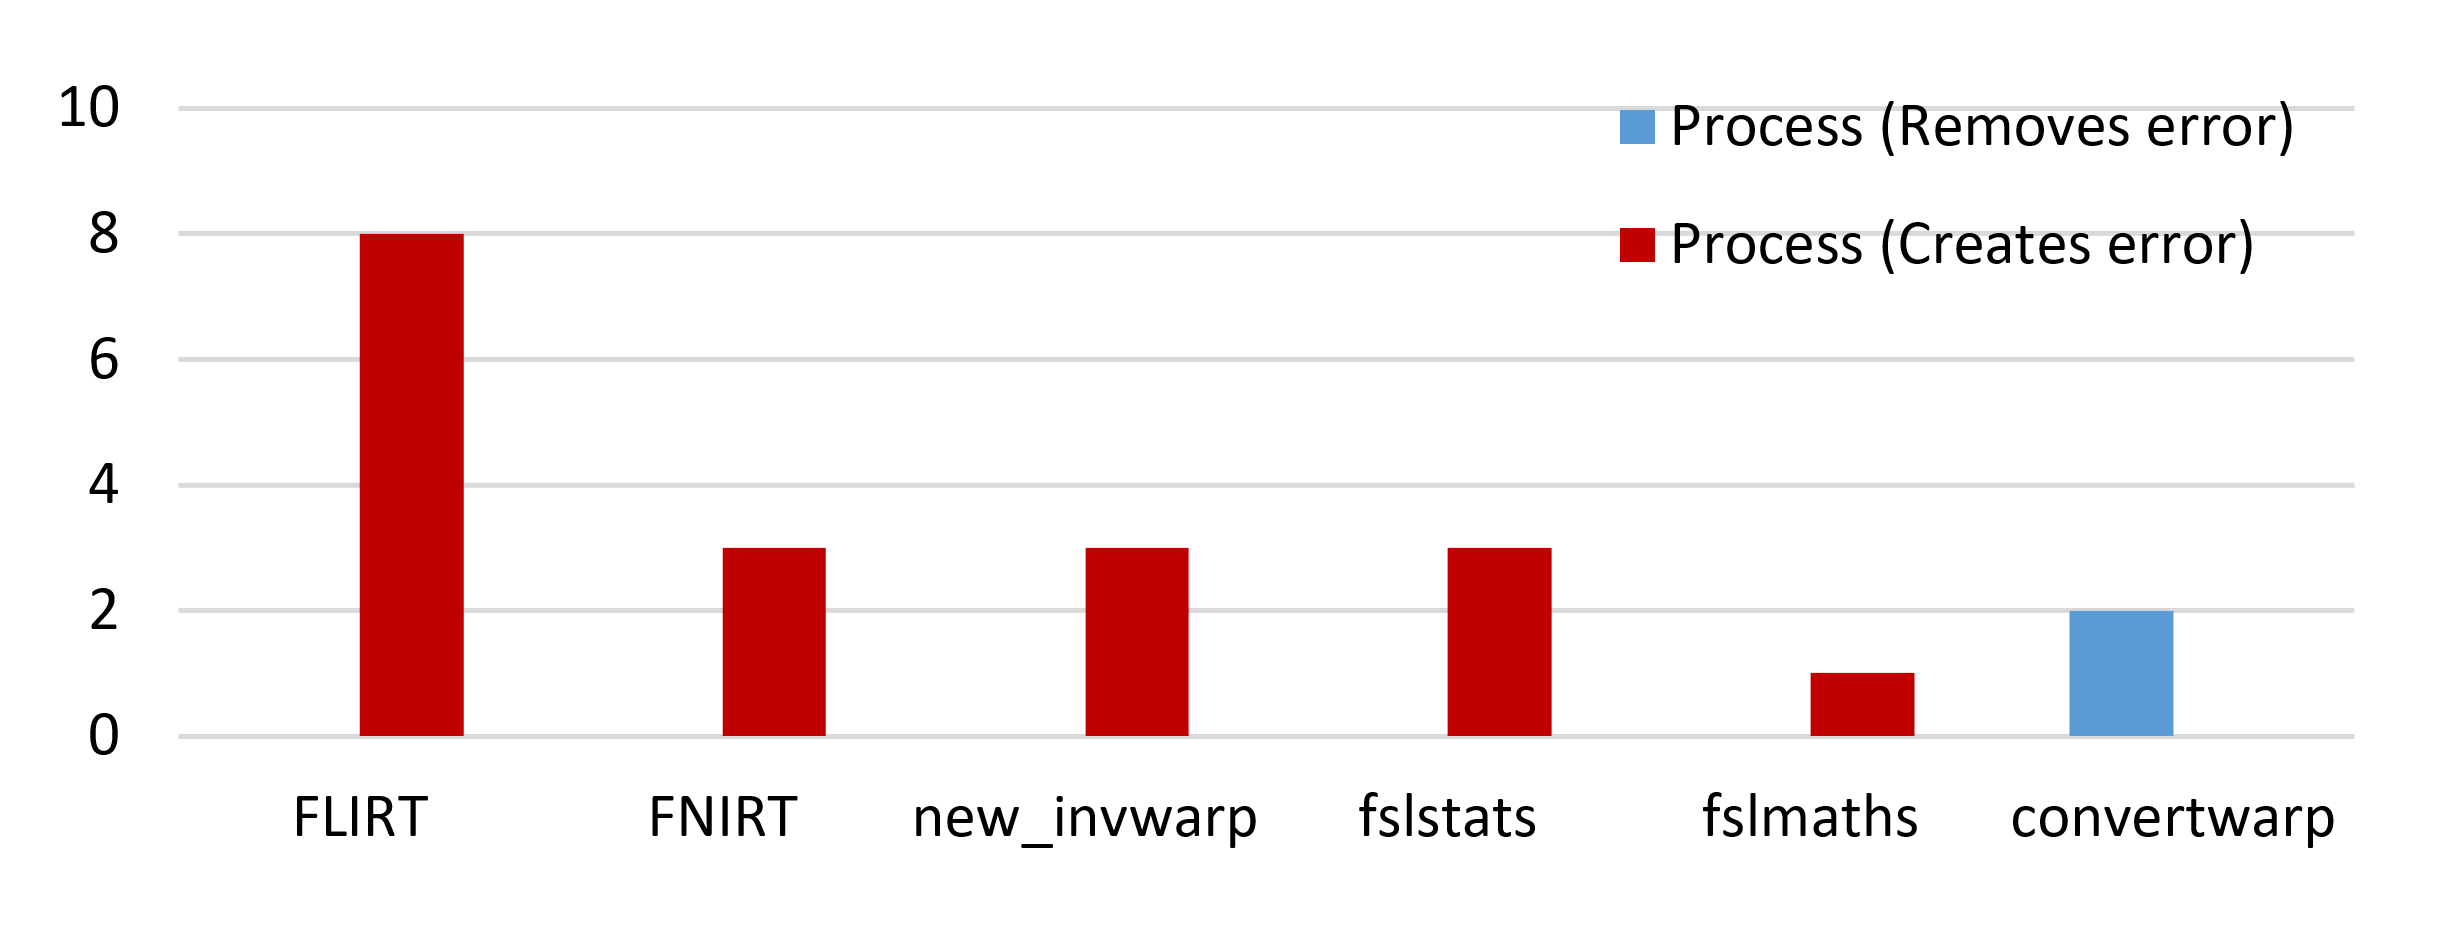
\includegraphics[scale=0.38]{images/pfs_chart.png} \caption{Number 
  of occurrences of errors in PreFreeSurfer on subject 103515, red and 
  blue bars indicate the processes which create and remove errors 
  respectively.} 
  \label{fig:pfs_chart}
\end{figure}


\paragraph{FreeSurfer.} In the second analysis, the result of 
PreFreeSurfer is considered as the input files of FreeSurfer pipeline. 
From the FreeSurfer results, total 61 files were found to be different 
between CentOS6 and CentOS7. The processes that introduce errors in 
FreeSurfer are shown on Figure~\ref{fig:fs_error_table}. Most frequent 
processes that create errors are \emph{mris\_anatomical\_stats} which 
measures a number of anatomical properties, \emph{mris\_make\_surface} 
to generate pial surfaces, first pass, no T2 adjustment, 
\emph{mri\_convert} which normalize T1w and T2w images for the benefit 
of \emph{mris\_make\_surfaces}, and \emph{fslmaths} create and apply a 
binary mask to filling of holes to remove  any non-grey/white tissue 
using a threshold created by FSLSTATS at Mean. In addition, all the 
other processes that created errors in the pipeline at least once are 
categorized as others such as \emph{mri\_ca\_register}, 
\emph{mri\_ca\_normalize}, and \emph{mri\_watershed}. Furthermore, 
processes that remove errors in FreeSurfer represented on 
Figure~\ref{fig:fs_remove_table} including \emph{mri\_convert} and 
\emph{mri\_surf2surf}. 

\begin{figure}[H] 
\centering
  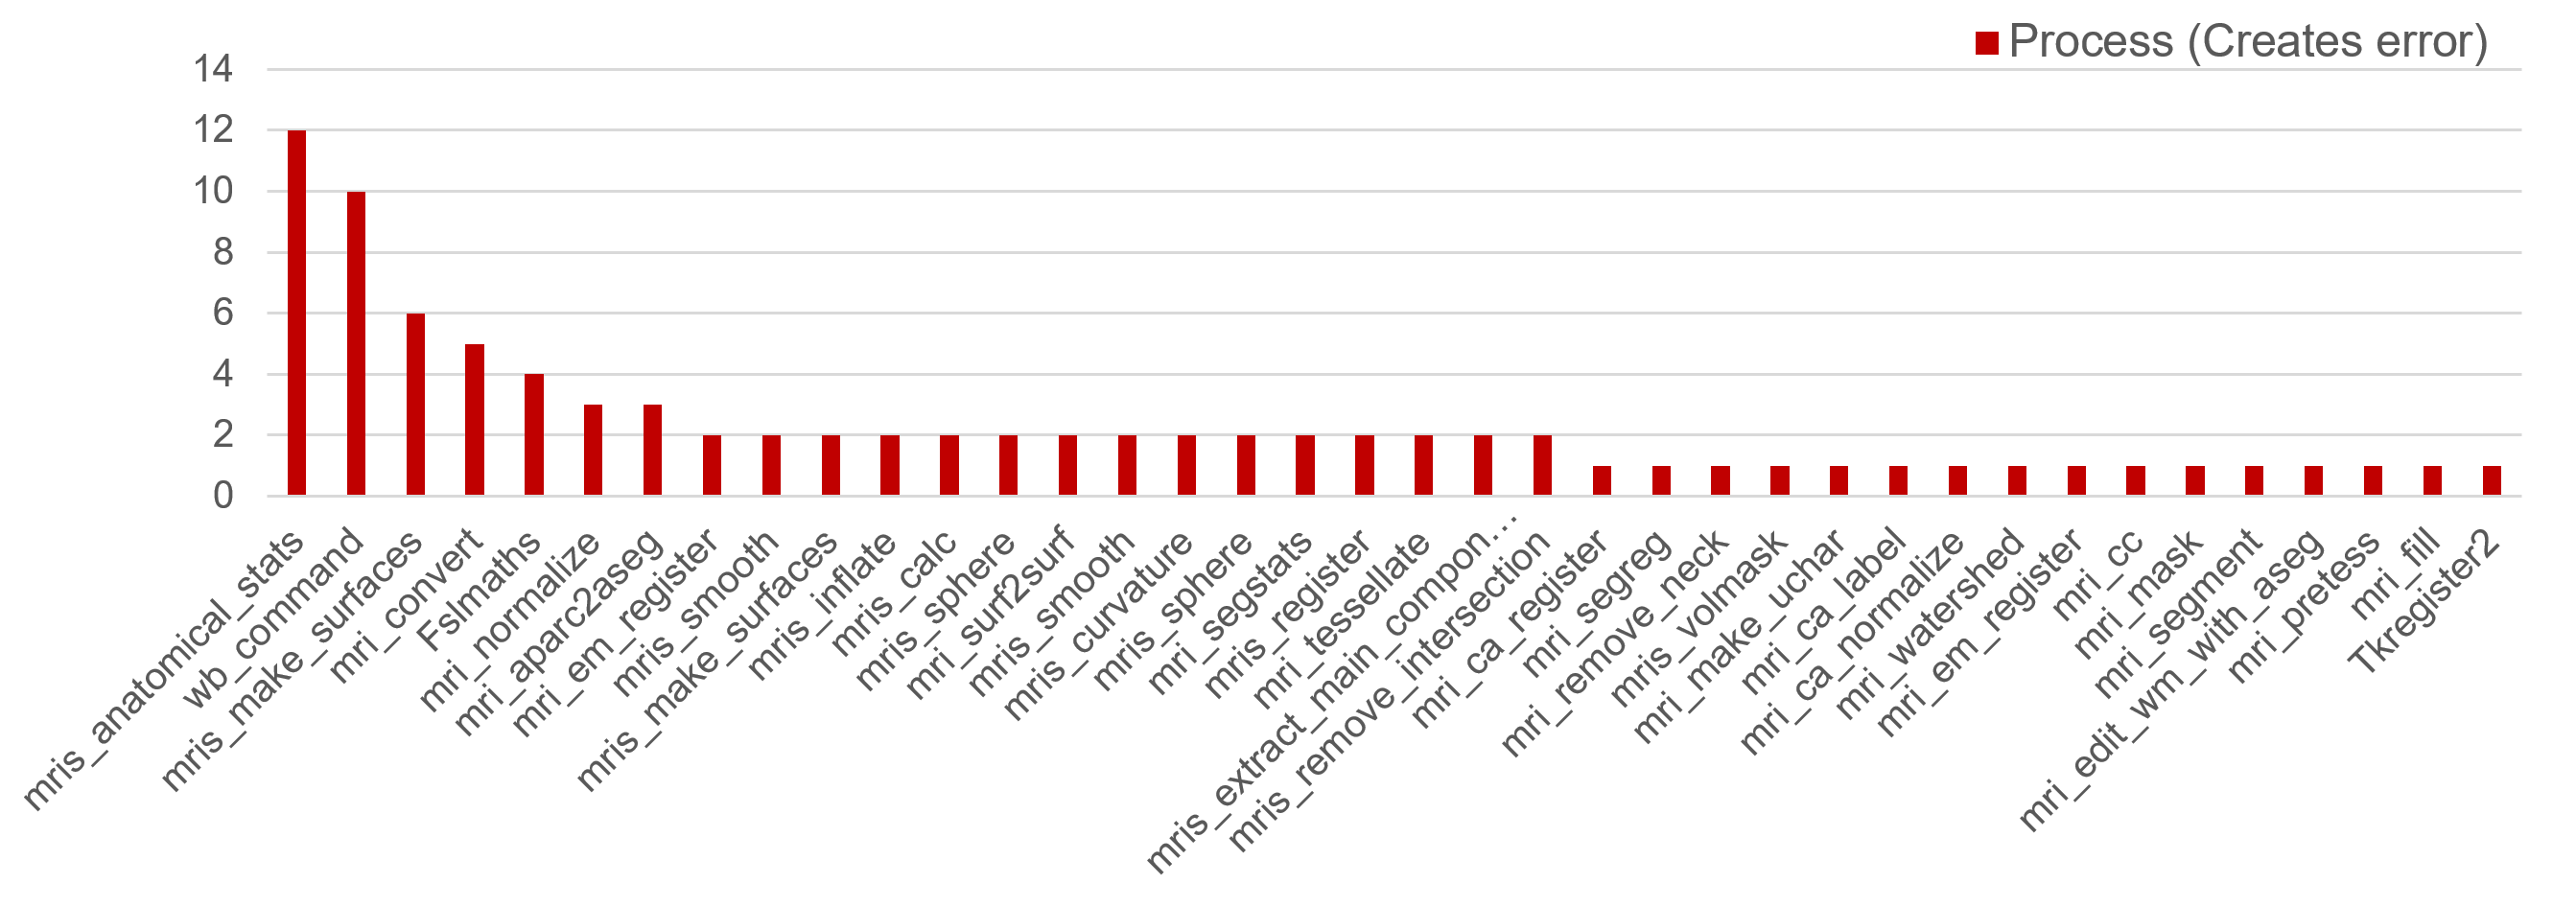
\includegraphics[scale=0.6]{images/fs_error_table.png} 
  \caption{Number of occurrences of errors in FreeSurfer pipeline, 
subject 103818, indicate the processes that create errors.}
  \label{fig:fs_error_table}
\end{figure}

\begin{figure}[H]
\centering
  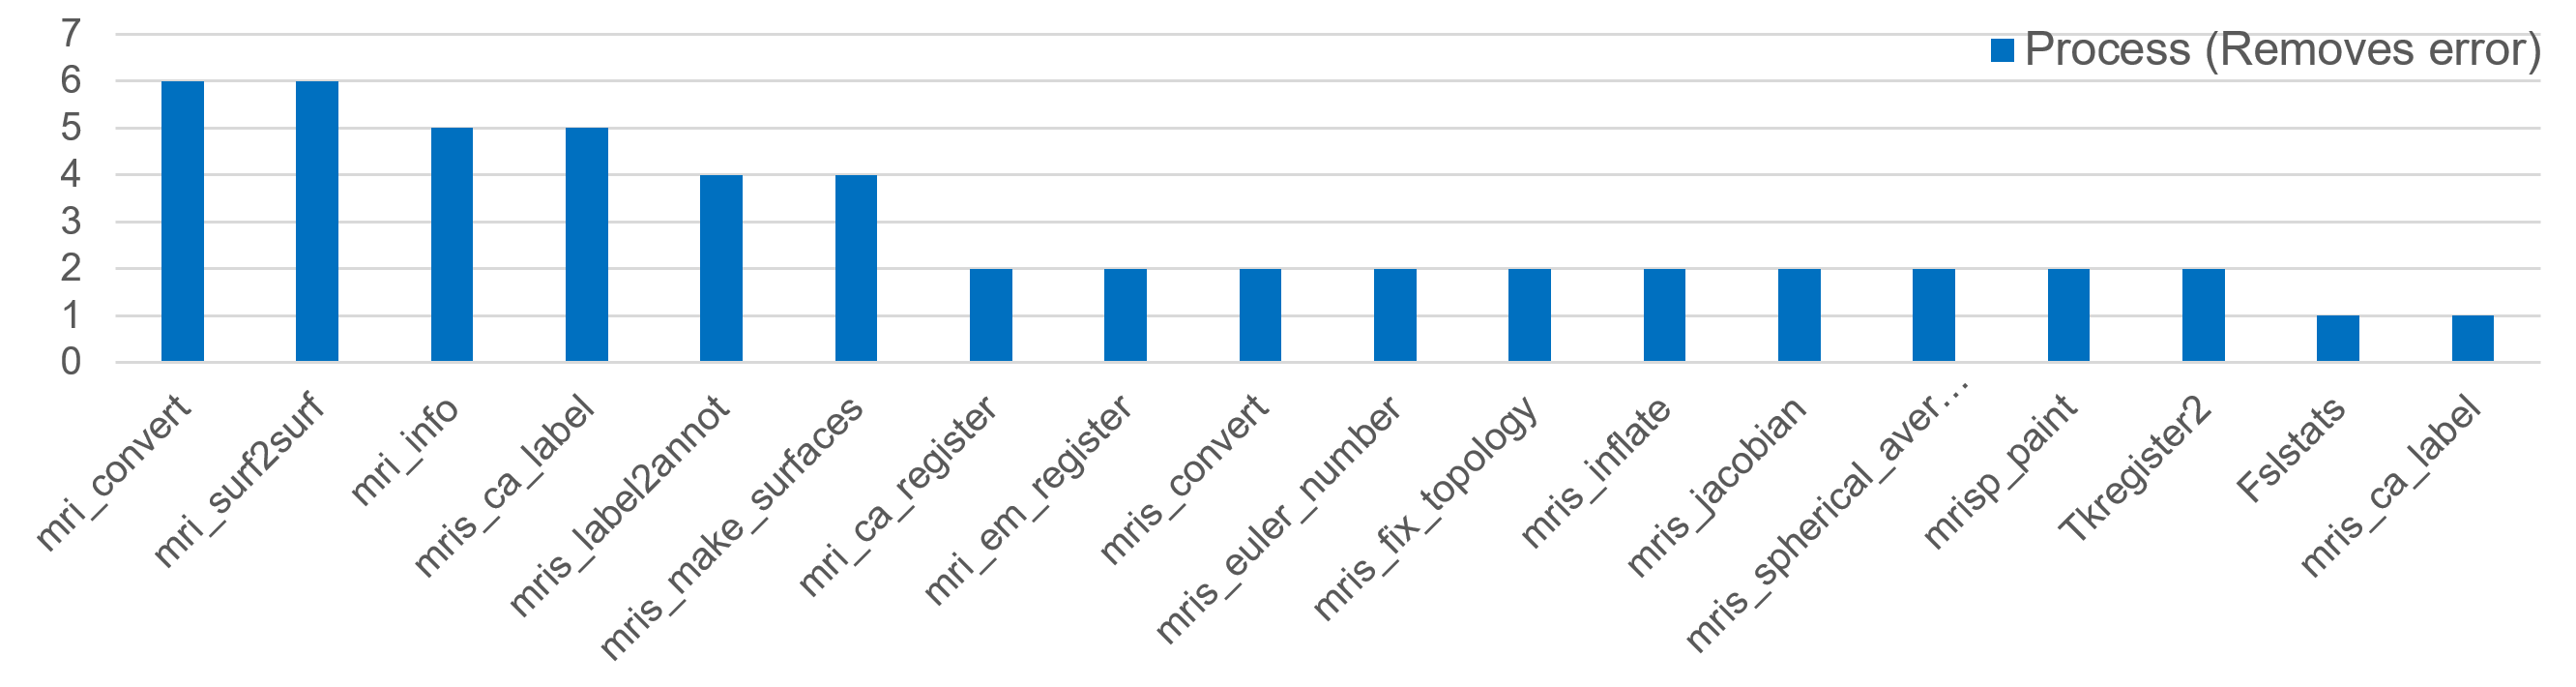
\includegraphics[scale=0.5]{images/fs_remove_table.png} 
  \caption{Number of occurrences of errors in FreeSurfer pipeline, 
subject 103818, indicate the processes that remove errors.}
  \label{fig:fs_remove_table}
\end{figure}


\section{Discussion}

pipeline amplify small numerical differences, they are numerically 
unstable. Furthermore, math libraries evolve over time, leading to 
different numerical errors. we listed some of the irreproducibility 
causes of the pipelines as we mentioned in the previous section 
overally along with exact command arguments.

Mention that this was only possible because the unprocessed data was shared in the first place.
DICOM to Nifti conversion was out of scope and may introduce other issues.

\section{Conclusion}

Our thechnique is able to characterize the stability of a pipeline's components automatically.
The numerical instability in the PreFreesurfer HCP pipeline arises mainly from
linear and non-linear registration processes implemented in FSL FLIRT and FNIRT. 

There are a few ways to impede such instabilities:
\begin{itemize}
\item Use a single operating system
\item Containerize pipelines
\item Increase numerical precision
\item Be stricter on truncation and rounding standards (IEEE 754)
\item Build static executable
\end{itemize}

The results still suffer from small pertubations literally because of the fact that pipeline are not numerically stable.
The preferred solution is to detect and fix numerical instability of the pipeline instead of masking the problem.
These processes need to be reviewed to understand and correct the cause of instabilities. 
In this correction process, accuracy has to be considered in addition to stability.

\item In the future works we aim to measure the impact of such errors
on the specific domain of the neuroscience and how show the significant it is.

\item The purpose of the project is generalizing pipelines to get a reproducible execution 
on every operating system instead of choosing one main OS to.


\section{Acknowledgments}

CBRAIN team. Compute Canada(Calcul Quebec).


\begin{figure}[H]
  \includegraphics[width=\linewidth]{images/summarized_graph}
  \caption{An annotated summarized process graph from the PreFreesurfer pipeline.
Each node in the graph is represented in red, blue or green colors and is labeled 
using the name of the executable run by the interesting process. The close up nodes 
reveal each shrinked subgraph in details.}
  \label{fig:summarized-graph}
\end{figure}

\begin{figure}[H]
  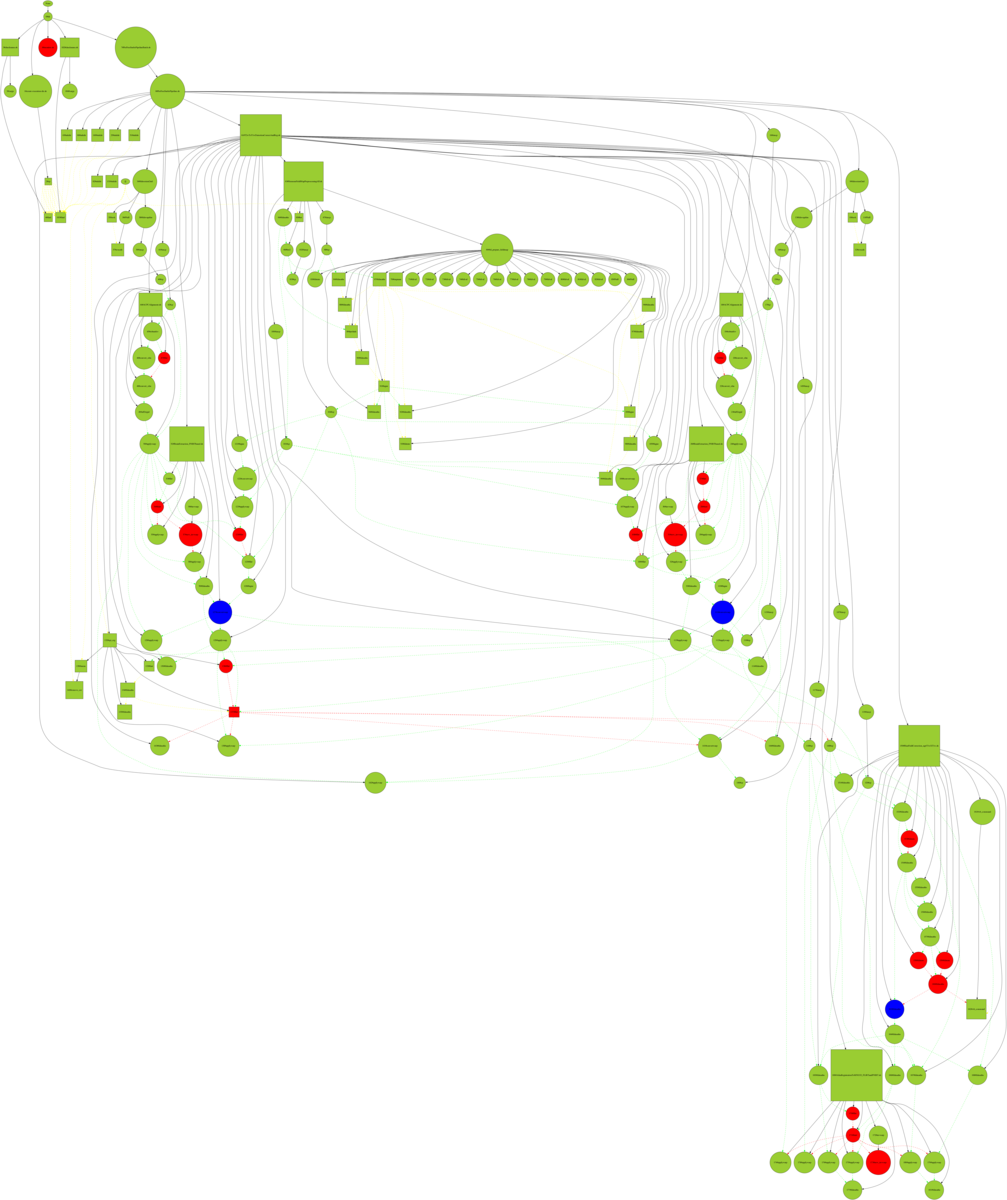
\includegraphics[width=\linewidth]{images/graph}
  \caption{A complete process graph from the PreFreesurfer pipeline.
Full-resolution image available at \url{https://drive.google.com/open?id=174yyn8SuVOUcK5aRVw0bagjDanLD0FLt}.}
  \label{fig:complete-graph}
\end{figure}
\bibliographystyle{plain}
\bibliography{biblio}

\end{document}
